\documentclass[11pt,a4paper]{article}

\usepackage[T1]{fontenc}
\usepackage[utf8]{inputenc}
\usepackage{lmodern}
\usepackage{microtype}
\usepackage[margin=2.5cm]{geometry}
\usepackage{amsmath,amssymb}
\usepackage{booktabs}
\usepackage{graphicx}
\usepackage{caption}
\usepackage{float}
\usepackage{setspace}
\usepackage[authoryear,round]{natbib}
\usepackage[colorlinks=true,linkcolor=black,citecolor=black,urlcolor=blue]{hyperref}

\captionsetup{font=small,labelfont=bf}
\setstretch{1.12}
\newcommand{\tabfit}[1]{\resizebox{\textwidth}{!}{\input{#1}}}

\title{\textbf{Momentum, Reversal, Volatility and Size in U.S.\ Large Caps:\\
A Cross-Sectional Factor Study with Fama-MacBeth Validation, 2011 to 2026}}
\author{Zack Higham\\[2pt]
\small BSc Mathematics (Statistics, Financial and AI pathway), Queen Mary University of London}
\date{September 2026}

\begin{document}
\maketitle

\begin{abstract}
\noindent
This paper tests whether four stock characteristics (12-1 momentum, one-month short-term reversal, 60-day realised volatility and log market capitalisation) predict the cross-section of monthly returns among the 200 largest current S\&P 500 constituents from 2011 to 2026. Each factor is evaluated through three complementary lenses: equal-weighted decile portfolio sorts, Fama-MacBeth cross-sectional regressions with Newey-West standard errors, and monthly rank information coefficients. The analysis is then stress-tested with a 60/40 in-sample and out-of-sample split, market risk adjustment, transaction costs, sector-neutral construction and a VIX regime split. In the joint Fama-MacBeth regression, momentum and volatility carry positive raw premia of 0.30\% and 0.49\% per month per cross-sectional standard deviation (Newey-West $t$ of 2.91 and 3.07), but risk adjustment separates them sharply. The volatility long-short portfolio has a market beta of 1.17 and a CAPM alpha that is insignificant over the full sample and negative before 2023, so its raw premium is largely compensation for market exposure in a strong bull market. Momentum is close to market-neutral, and its market-adjusted Fama-MacBeth premium of 3.7\% a year per standard deviation is significant ($t = 3.41$), including before 2023 ($t = 2.49$). Short-term reversal is indistinguishable from zero after costs. The strongly negative size premium, and a positive residual volatility premium that contradicts the literature, are attributed to survivorship bias in a universe selected on end-of-sample market capitalisation. The contribution is methodological rather than a claim of a tradable edge: a transparent, reproducible pipeline that separates what the data support from what market exposure and sample construction manufacture.
\end{abstract}

\section{Introduction}

Cross-sectional factor research asks a simple question: do stocks that share a measurable characteristic today earn systematically different returns next month? The question underpins most systematic equity strategies, and the standard tools for answering it are portfolio sorts and the two-step regression procedure of \citet{fama1973}. This paper applies both, alongside rank information coefficients, to four characteristics with a long empirical history.

\textbf{Momentum.} \citet{jegadeesh1993} document that stocks with high returns over the prior three to twelve months continue to outperform. The standard 12-1 construction skips the most recent month to separate momentum from short-term reversal \citep{carhart1997}. \citet{daniel2016} show that momentum is prone to sharp crashes when markets rebound after a decline.

\textbf{Short-term reversal.} \citet{jegadeesh1990} and \citet{lehmann1990} find that short-horizon winners (over the prior month and prior week respectively) tend to underperform subsequently, an effect usually attributed to liquidity provision and microstructure, and concentrated in smaller, less liquid stocks.

\textbf{Volatility.} \citet{ang2006} report that high idiosyncratic volatility stocks earn low subsequent returns, and \citet{baker2011} and \citet{frazzini2014} relate the low-risk anomaly to leverage constraints and benchmarking. A positive volatility premium would therefore contradict the classic anomaly and requires explanation.

\textbf{Size.} \citet{banz1981} and \citet{fama1992} find that small firms earn higher average returns. Here size mainly serves as a control variable, and Section~\ref{sec:limitations} explains why its estimated premium in this universe cannot be interpreted at face value.

The paper makes three points. First, the three evaluation lenses disagree in informative ways, and the disagreements identify where each factor's predictive content sits in the cross-section. Second, raw premia can be badly misleading in a strong bull market: the most significant raw result, the volatility premium, is largely market beta, while momentum's premium only becomes clearly robust once market exposure is removed. Third, several results are products of the research design itself (survivorship bias from selecting the universe at the end of the sample), and a credible factor study has to identify these before claiming any premium. Given the well-documented problem of multiple testing in factor research \citep{harvey2016} and post-publication decay of anomalies \citep{mclean2016}, the paper favours conservative interpretation throughout.

\section{Data}
\label{sec:data}

\textbf{Universe.} The universe is the 200 largest constituents of the S\&P 500 by market capitalisation as of September 2026, taken from the current Wikipedia constituent list with GICS sector labels, and ranked using Yahoo Finance market capitalisations (from \$58.6 billion to \$5.17 trillion). The universe spans all 11 GICS sectors, from 39 Information Technology stocks to 5 Utilities. Because membership is fixed at the end of the sample, the universe is survivorship-biased by construction; the consequences are quantified in Section~\ref{sec:limitations}.

\textbf{Prices.} Daily dividend- and split-adjusted closing prices were downloaded from Yahoo Finance for 3,949 trading days from 3 January 2011 to 16 September 2026. Month-end prices are the last available close in each month. Because the price series ends mid-month, the incomplete September 2026 return is excluded, so the return sample ends in August 2026. Nineteen of the 200 stocks have less than 90\% daily coverage because they listed or were spun off during the sample (for example AbbVie, Hewlett Packard Enterprise and Vertiv). A stock enters a factor only once it has enough history, so these late entrants account for 1,806 missing momentum observations, 5.2\% of the momentum stock-month panel.

\textbf{Market data.} The market benchmark is the SPDR S\&P 500 ETF (SPY), using dividend-adjusted prices as a total-return proxy, and the risk-free rate is the 13-week U.S.\ Treasury bill yield, both from Yahoo Finance. SPY holds the index constituents as they were at each point in time, so unlike an average of this paper's universe it is free of the universe's survivorship bias. The CBOE VIX index is used for the regime analysis.

\textbf{Data validation.} Before any factor was built, the price panel was checked for empty series, internal gaps and single-day moves above 50\%. No series has internal gaps. Seven extreme daily moves were identified and six were verified against real events (for example the March 2020 oil price collapse and biotech trial readouts); none was treated as an error. Table~\ref{tab:factor_summary} summarises the resulting factor panels.

\begin{table}[H]
\centering
\caption{Factor panels. Pooled statistics across all stock-months after winsorisation (size is not winsorised). Momentum and reversal are simple returns, volatility is annualised, size is the natural log of market capitalisation in U.S.\ dollars.}
\label{tab:factor_summary}
\small
\begin{tabular}{lrrrrrrr}
\toprule
Factor & First month & Months & Avg.\ stocks & Mean & Std.\ dev. & P1 & P99 \\
\midrule
Momentum & 2012-02 & 176 & $189$ & $0.193$ & $0.368$ & $-0.412$ & $1.356$ \\
Reversal & 2011-03 & 187 & $190$ & $0.016$ & $0.082$ & $-0.182$ & $0.246$ \\
Volatility & 2011-04 & 186 & $190$ & $0.279$ & $0.145$ & $0.108$ & $0.838$ \\
Size & 2011-02 & 188 & $190$ & $24.618$ & $1.164$ & $22.065$ & $28.048$ \\
\bottomrule
\end{tabular}

\end{table}

\section{Methodology}
\label{sec:method}

\subsection{Timing convention}

Let $P_{i,t}$ be the adjusted month-end price of stock $i$ in month $t$. The return to be predicted is the return earned during month $t$,
\begin{equation}
R_{i,t} = \frac{P_{i,t}}{P_{i,t-1}} - 1 .
\end{equation}
Every factor value paired with $R_{i,t}$ uses only information available at the close of month $t-1$. This single convention is applied to all factors and all tests, and it is the main safeguard against look-ahead bias. It was verified by recomputing individual factor values and returns by hand for sample stocks and months.

\subsection{Factor definitions}

\begin{align}
\text{MOM}_{i,t} &= \frac{P_{i,t-2}}{P_{i,t-13}} - 1 && \text{(12-1 momentum: months } t-12 \text{ to } t-2\text{)}\\
\text{REV}_{i,t} &= \frac{P_{i,t-1}}{P_{i,t-2}} - 1 && \text{(short-term reversal: month } t-1\text{)}\\
\text{VOL}_{i,t} &= \sqrt{252}\;\operatorname{sd}\big(r_{i,d}\big)_{d \in \mathcal{D}_{t-1}} && \text{(realised volatility)}\\
\text{SIZE}_{i,t} &= \ln\big(S_i \, P_{i,t-1}\big) && \text{(log market capitalisation)}
\end{align}
Here $r_{i,d}$ are daily simple returns and $\mathcal{D}_{t-1}$ is the 60 trading days ending on the last trading day of month $t-1$. The momentum and reversal windows do not overlap, so the two factors measure distinct horizons. Historical shares outstanding are not available from the data source, so market capitalisation uses the current share count $S_i$ throughout, which ignores buybacks and issuance.

\subsection{Winsorisation}

Momentum, reversal and volatility are winsorised cross-sectionally each month at the 1st and 99th percentiles, which alters 2.11\% of observations for each factor. Winsorising each month rather than against a single global cut-off keeps the thresholds appropriate for the volatility regime of that month. The upper tail contained genuine but extreme values (for example a 12-1 momentum reading of more than 5,000\% for SanDisk in 2026); the lower tail contained artificially low values (Vertiv's near-constant price during its pre-merger SPAC period implied almost zero volatility). Size is not winsorised because the log transform already compresses its scale. Returns are never winsorised, so portfolio performance is not artificially smoothed.

\subsection{Decile portfolios and turnover}

Each month, stocks are ranked on each factor and assigned to deciles using the cross-sectional percentile rank $u_{i,t} \in (0,1]$, with decile $\lceil 10\,u_{i,t} \rceil$. Months with fewer than 100 valid stocks are excluded. Each decile is equal-weighted and held for one month. The long-short portfolio is always decile 10 minus decile 1 (high minus low), so that a negative spread means the factor is negatively related to future returns, matching the sign of the regression coefficients.

Long-short weights are $w_{i,t} = 1/n^{10}_t$ for decile 10 stocks, $-1/n^{1}_t$ for decile 1 stocks and zero otherwise. Turnover is
\begin{equation}
\text{TO}_t = \sum_i \big| w_{i,t} - w_{i,t-1} \big| ,
\end{equation}
which ranges from 0 (no change) to 4 (both legs entirely replaced). Weights are reset to equal each month, so drift in weights within the month is ignored.

\subsection{Fama-MacBeth regressions}

In the first step, for each month $t$ with at least 100 stocks with complete data, the cross-section of returns is regressed on the factors:
\begin{equation}
R_{i,t} = a_t + \sum_{k} \gamma_{k,t}\, z_{k,i,t} + \varepsilon_{i,t},
\end{equation}
where $z_{k,i,t}$ is factor $k$ standardised to zero mean and unit standard deviation across the stocks in that month's regression. Standardisation makes $\gamma_{k,t}$ the return premium, in that month, for a one standard deviation higher exposure to factor $k$, comparable across factors and over time. Factors are estimated both one at a time (univariate) and jointly (multivariate), where each slope measures the premium holding the other factors fixed.

In the second step, the premium estimate is the time-series mean $\bar\gamma_k = T^{-1}\sum_t \gamma_{k,t}$. The classic Fama-MacBeth standard error, $\operatorname{sd}(\gamma_{k,t})/\sqrt{T}$, assumes the monthly slopes are serially uncorrelated. Slowly moving characteristics such as momentum and size can make consecutive slopes correlated, so inference uses Newey-West heteroskedasticity and autocorrelation consistent standard errors \citep{newey1987} with a Bartlett kernel and $L = \lfloor 4 (T/100)^{2/9} \rfloor = 4$ lags \citep{newey1994}. Plain Fama-MacBeth $t$-statistics are reported alongside for comparison. As a check on the implementation, the monthly slopes were recomputed independently with a direct least-squares solve and matched exactly.

\subsection{Market risk adjustment}

A long-short spread can be positive simply because its long leg has a higher market beta than its short leg, which pays off whenever the market rises. Two complementary adjustments address this. First, each long-short return series is regressed on the market excess return,
\begin{equation}
\text{LS}_{t} = \alpha + \beta\,\big(R_{m,t} - r_{f,t}\big) + e_t ,
\end{equation}
where $R_{m,t}$ is the SPY return and $r_{f,t}$ is the Treasury bill yield at the end of month $t-1$ divided by 12. Because a long-short portfolio is self-financing, its return is already an excess return. The CAPM alpha $\alpha$ \citep{sharpe1964} is the return not explained by market exposure; it is annualised and tested with Newey-West standard errors.

Second, each stock's market beta is added to the Fama-MacBeth regressions as a fifth characteristic. Beta is the slope of the stock's daily returns on SPY's daily returns over the trailing 252 trading days, measured at the end of month $t-1$ and winsorised like the other factors. Controlling for beta as a characteristic is not the same as hedging the market, because each monthly slope $\gamma_{k,t}$ is itself the return of a factor-mimicking portfolio that can still load on the market. The monthly slope series are therefore also regressed on the market excess return, which gives a market-adjusted premium for each factor.

\subsection{Information coefficient}

The information coefficient (IC) for factor $k$ in month $t$ is the Spearman rank correlation across stocks between $f_{k,i,t}$ and $R_{i,t}$ \citep{grinold2000}. The IC measures how well a factor orders stocks, uses every stock equally and is insensitive to outliers. The annualised information ratio of the IC is $\text{ICIR} = \sqrt{12}\,\overline{\text{IC}}/\operatorname{sd}(\text{IC})$.

\subsection{Validation design}

\textbf{Out-of-sample split.} The 175-month sample in which all four factors are available (February 2012 to August 2026) is split at one calendar date for every factor: the first 60\% (105 months, to October 2020) is in-sample and the remaining 70 months are out-of-sample. Because no parameter is estimated in-sample (all factor definitions are fixed in advance from the literature), the split tests the stability of the premia over time rather than overfitting in the usual sense.

\textbf{Transaction costs.} Net returns deduct $c \cdot \text{TO}_t$ each month with $c = 10$ basis points per unit of turnover, and the first month is charged the full initial build ($\text{TO} = 2$). Sensitivity to $c \in \{0, 5, 10, 20\}$ basis points and the break-even cost $\bar R^{\text{gross}} / \overline{\text{TO}}$ are reported.

\textbf{Sector neutrality.} Several sectors contain too few stocks for deciles within each sector (the smallest has five), so each stock's factor value is first converted to a percentile rank within its GICS sector and deciles are then formed on the pooled within-sector ranks. Each decile then holds approximately the universe's sector mix. The regression counterpart adds sector dummy variables, so that slopes are identified only from differences between stocks in the same sector.

\textbf{VIX regimes.} Each month $t$ is classified by the VIX close at the end of month $t-1$, split into terciles over the full sample (cut-offs 14.8 and 18.2; 58, 59 and 58 months). Because the cut-offs use the whole sample, this is a descriptive conditioning analysis, not a tradable timing rule. Differences between high- and low-VIX months are tested with Welch's unequal-variance $t$-test.

\section{Results}
\label{sec:results}

\subsection{Decile portfolios}

Table~\ref{tab:decile_means} and Figure~\ref{fig:deciles} show mean monthly returns by decile. The volatility sort is close to monotonic, with decile 10 earning 3.13\% per month against 1.20\% for decile 1. The momentum and reversal sorts are U-shaped rather than monotonic: both extreme deciles outperform the middle of the distribution. This pattern reflects a nonlinear relationship between the factors: stocks with extreme past returns, whether winners or losers, tend to be high-volatility stocks (average volatility is 0.36 in both momentum decile 1 and decile 10, against about 0.24 in deciles 4 to 7), so the extreme momentum and reversal deciles partly inherit the volatility effect. The average cross-sectional rank correlation between momentum and volatility is close to zero, because a U-shaped relationship is invisible to a linear correlation measure.

\begin{table}[H]
\centering
\caption{Mean monthly return (\%) of equal-weighted decile portfolios. D1 holds the lowest factor values, D10 the highest.}
\label{tab:decile_means}
\small
\tabfit{tables/decile_means}
\end{table}

\begin{figure}[H]
\centering
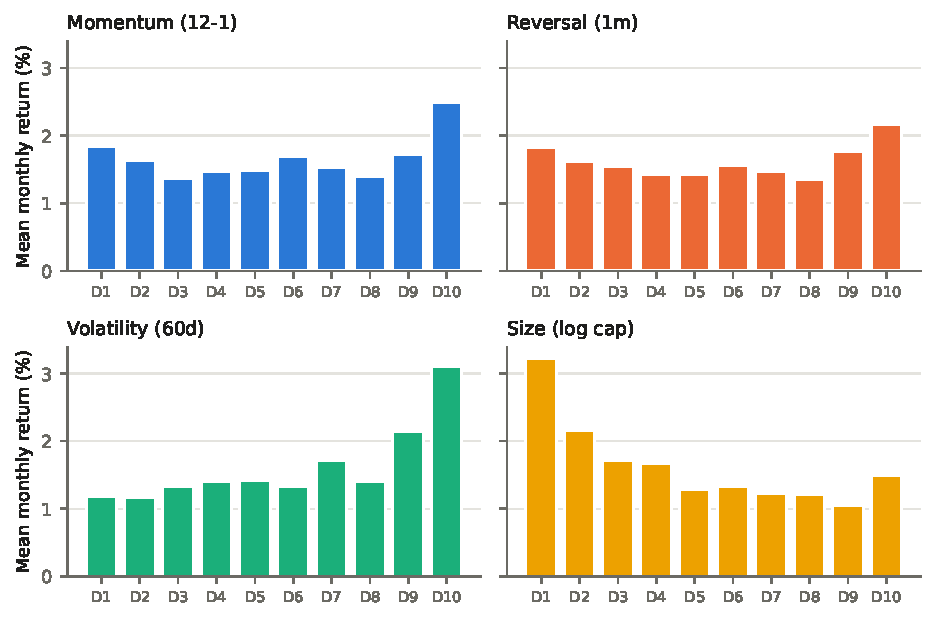
\includegraphics[width=\textwidth]{figures/decile_returns.pdf}
\caption{Mean monthly return by decile. Volatility is close to monotonic; momentum and reversal are U-shaped; size falls from D1 to D9.}
\label{fig:deciles}
\end{figure}

Table~\ref{tab:decile_spreads} reports the long-short spreads. Only volatility (Newey-West $t = 2.83$) and size ($t = -4.92$) are significant. The momentum spread earns 7.31\% a year gross with a Sharpe ratio of 0.29 and is not significant ($t = 1.18$); the U-shape means the short leg of losers performs well and erodes the spread. Figure~\ref{fig:cumulative} shows the cumulative performance of each spread.

\begin{table}[H]
\centering
\caption{Decile 10 minus decile 1 long-short portfolios, gross of costs. Newey-West $t$-statistic on the mean monthly return with 4 lags. Turnover is the mean monthly $\text{TO}_t$ (maximum 4).}
\label{tab:decile_spreads}
\small
\tabfit{tables/decile_spreads}
\end{table}

\begin{figure}[H]
\centering
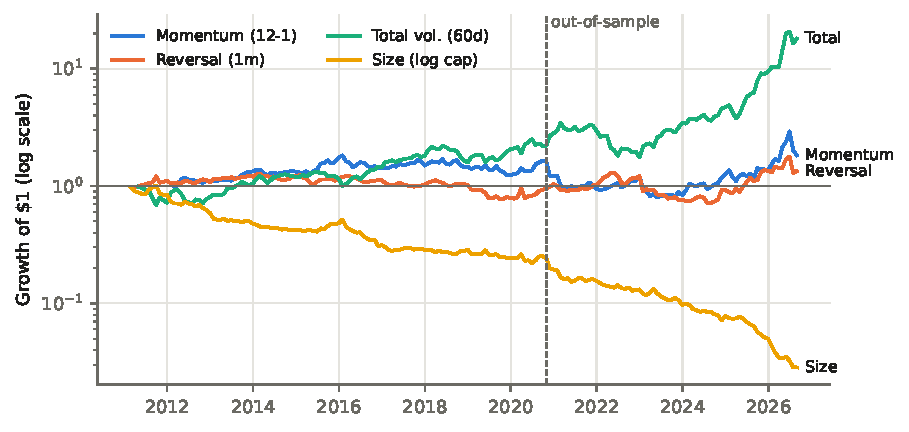
\includegraphics[width=\textwidth]{figures/cumulative_long_short.pdf}
\caption{Growth of \$1 in each long-short portfolio (gross, log scale). The dashed line marks the start of the out-of-sample period (November 2020).}
\label{fig:cumulative}
\end{figure}

\subsection{Fama-MacBeth regressions}

Table~\ref{tab:fm} reports the regression results. In the multivariate specification, momentum earns 0.30\% per month per standard deviation ($t = 2.91$) and volatility 0.49\% ($t = 3.07$); reversal is insignificant ($t = 0.51$) and size is negative ($t = -3.85$). The monthly regressions explain on average 14.5\% of cross-sectional return variation across an average of 189 stocks.

Three features of the table deserve comment. First, momentum is significant in the regression but not in the decile sort. The regression uses every stock with a linear weight, while the sort uses only the two extreme deciles, where the U-shape works against the spread. Second, the momentum premium barely changes between the univariate and multivariate specifications (0.285\% and 0.296\%); its $t$-statistic rises because the other factors absorb cross-sectional noise and reduce the variance of the monthly slopes. Controlling for volatility linearly does not remove the nonlinear overlap seen in the decile sorts. Third, Newey-West and plain $t$-statistics are similar, which indicates only modest autocorrelation in the monthly slopes. Figure~\ref{fig:fm} plots the slopes over time.

\begin{table}[H]
\centering
\caption{Fama-MacBeth regressions of monthly returns on standardised factors. $\bar\gamma$ is the mean monthly slope in \% per one cross-sectional standard deviation. Newey-West $t$-statistics (4 lags) in parentheses. Multivariate sample: 175 months, February 2012 to August 2026.}
\label{tab:fm}
\small
\tabfit{tables/fama_macbeth}
\end{table}

\begin{figure}[H]
\centering
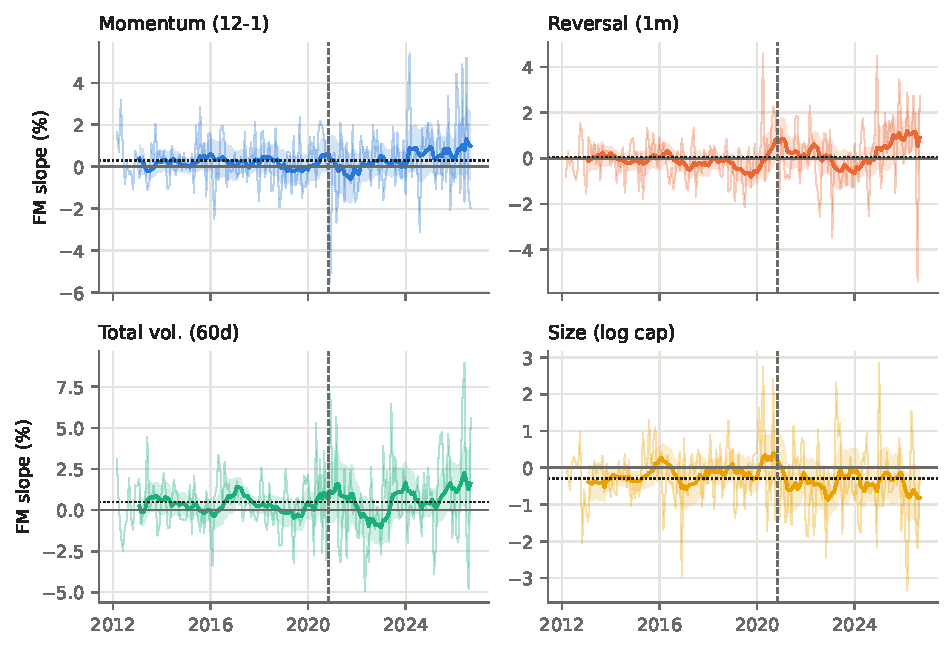
\includegraphics[width=\textwidth]{figures/fm_coefficients.pdf}
\caption{Monthly multivariate Fama-MacBeth slopes (faint), their 12-month rolling mean (solid) with a 95\% band, and the full-sample mean (dotted). The dashed line marks the out-of-sample split.}
\label{fig:fm}
\end{figure}

\subsection{Information coefficients}

Table~\ref{tab:ic} reports rank ICs. Only size has a significant mean IC. The mean ICs for momentum (0.010) and volatility (0.028) are small and insignificant, and momentum's IC is positive in only 50.9\% of months. Figure~\ref{fig:ic} shows the IC over time.

\begin{table}[H]
\centering
\caption{Monthly Spearman rank information coefficients between factor values and next-month returns. Newey-West $t$ on the mean IC (4 lags).}
\label{tab:ic}
\small
\begin{tabular}{lrrrrrr}
\toprule
Factor & Months & Mean IC & IC std.\ dev. & ICIR (ann.) & NW $t$ & \% months IC $>0$ \\
\midrule
Momentum & 176 & $0.011$ & $0.210$ & $0.18$ & $0.80$ & $51.1$ \\
Reversal & 187 & $-0.002$ & $0.179$ & $-0.03$ & $-0.14$ & $47.6$ \\
Volatility & 186 & $0.028$ & $0.256$ & $0.38$ & $1.55$ & $54.3$ \\
Size & 188 & $-0.059$ & $0.145$ & $-1.41$ & $-5.93$ & $34.0$ \\
\bottomrule
\end{tabular}

\end{table}

\begin{figure}[H]
\centering
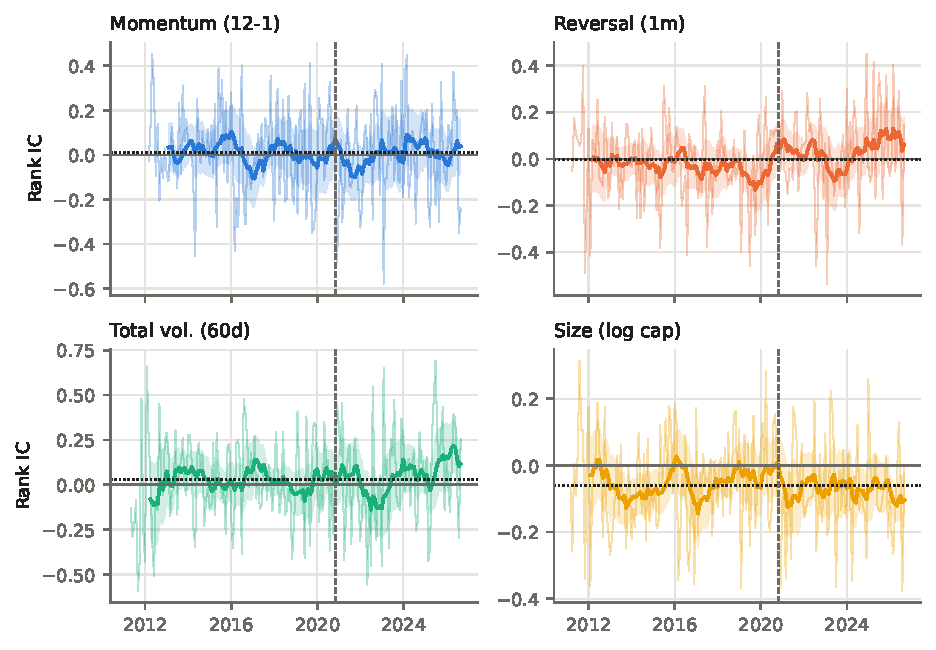
\includegraphics[width=\textwidth]{figures/ic_timeseries.pdf}
\caption{Monthly rank IC (faint) and its 12-month rolling mean with a 95\% band.}
\label{fig:ic}
\end{figure}

\subsection{Reconciling the three lenses}

The lenses answer different questions. The IC asks whether a factor orders all stocks correctly, giving each stock equal weight. The regression asks whether return is linearly related to the factor's magnitude, so extreme observations carry more weight. The decile spread asks whether the extreme deciles differ. For momentum and volatility the regression is significant while the IC is not, which means the predictive content is concentrated in the tails of the cross-section (a handful of extreme stocks) rather than spread evenly across all 200 names. Section~\ref{sec:robust} examines whether these premia are stable over time and whether they survive adjustment for market exposure.

\section{Robustness and Validation}
\label{sec:robust}

\subsection{Out-of-sample and subperiod stability}

Table~\ref{tab:is_oos} compares the two halves of the sample. Momentum's regression premium is significant in-sample ($t = 2.46$) but not out-of-sample ($t = 1.80$), and the annualised volatility of its long-short portfolio roughly doubles from 16.6\% to 33.9\%. Volatility is significant in both halves, but its long-short return rises from 12.61\% to 43.68\% a year, which is not a plausible stationary premium.

\begin{table}[H]
\centering
\caption{In-sample and out-of-sample comparison: long-short annualised return and Sharpe ratio (gross), and multivariate Fama-MacBeth premia with Newey-West $t$-statistics.}
\label{tab:is_oos}
\small
\tabfit{tables/is_oos}
\end{table}

A split at the end of 2022 is more revealing (Table~\ref{tab:subperiods}). Before 2023, neither raw premium is significant at the 5\% level (momentum $t = 1.87$, volatility $t = 1.56$). From 2023 to August 2026, a period of 44 months dominated by the rally in AI, memory and semiconductor stocks, both raw premia are three to five times larger, and the volatility long-short portfolio earned 6.06\% per month against 0.64\% before 2023. Two explanations compete for this concentration: a genuine market episode, and the fact that the universe is selected on September 2026 market capitalisation, so that selection is strongest for stocks whose value rose most in the final years (SanDisk, for example, is in the universe only because of its 2025 to 2026 rise). Section~\ref{sec:risk} shows that once market exposure is removed, the picture differs sharply between the two factors.

\begin{table}[H]
\centering
\caption{Multivariate Fama-MacBeth premia before and during the 2023 to 2026 rally.}
\label{tab:subperiods}
\small
\begin{tabular}{lrrrr}
\toprule
& \multicolumn{2}{c}{2012-02 to 2022-12 (131 months)} & \multicolumn{2}{c}{2023-01 to 2026-08 (44 months)} \\
\cmidrule(lr){2-3} \cmidrule(lr){4-5}
Factor & $\bar\gamma$ (\%) & NW $t$ & $\bar\gamma$ (\%) & NW $t$ \\
\midrule
Momentum & $0.191$ & $(1.87)$ & $0.608$ & $(2.48)$ \\
Reversal & $-0.028$ & $(-0.30)$ & $0.283$ & $(1.14)$ \\
Total volatility & $0.251$ & $(1.56)$ & $1.216$ & $(3.28)$ \\
Size & $-0.237$ & $(-2.94)$ & $-0.414$ & $(-2.52)$ \\
\bottomrule
\end{tabular}

\end{table}

Momentum's worst months (Table~\ref{tab:crashes}) include November 2020 and February 2021, both following months of elevated VIX (38.0 and 33.1). These match the rebound crashes described by \citet{daniel2016}, in which past losers rally sharply as markets recover. The worst month, July 2026, occurred at a low VIX and was a sharp reversal within the semiconductor rally itself: the winner decile, led by SanDisk, Corning, KLA, Marvell and Intel, fell 20.9\% while the loser decile rose 10.4\%.

\begin{table}[H]
\centering
\caption{The five worst monthly returns of the momentum long-short portfolio.}
\label{tab:crashes}
\small
\begin{tabular}{lrr}
\toprule
Month & Momentum L/S return (\%) & VIX at prior month-end \\
\midrule
2026-07 & $-31.4$ & $16.5$ \\
2020-11 & $-24.3$ & $38.0$ \\
2023-01 & $-19.8$ & $21.7$ \\
2021-02 & $-16.8$ & $33.1$ \\
2025-02 & $-11.7$ & $16.4$ \\
\bottomrule
\end{tabular}

\end{table}

\subsection{Market risk adjustment}
\label{sec:risk}

Table~\ref{tab:capm} reports CAPM regressions of the long-short portfolios on the SPY excess return. The volatility spread is a leveraged market position: its beta is 1.17 ($t = 6.99$) and the regression explains 30\% of its variance. Its CAPM alpha of 8.30\% a year is not significant ($t = 1.31$) and is negative before 2023 ($-3.13\%$, $t = -0.54$); all of the remaining alpha comes from 2023 to 2026 (38.80\% a year). Over the long-run part of the sample, the high-minus-low volatility spread is therefore explained by market exposure. Momentum behaves in the opposite way. Its beta is slightly negative over the full sample, its alpha of 8.97\% a year is earned mainly before 2023, and its raw strength after 2023 came with a beta of 0.89, because the winner decile in that period consisted largely of high-beta technology stocks. Momentum's decile alphas are only marginally significant across specifications ($t$ between 1.46 and 1.71), consistent with the noise of 20-stock deciles and the U-shape discussed in Section~\ref{sec:results}.

\begin{table}[H]
\centering
\caption{CAPM regressions of long-short portfolios on the SPY excess return. Beta is from the full-sample gross regression. Alphas are annualised with Newey-West $t$-statistics (4 lags) in parentheses. Net alphas deduct 10 basis points per unit turnover.}
\label{tab:capm}
\small
\tabfit{tables/capm_alphas}
\end{table}

Table~\ref{tab:fmrisk} turns to the regressions. Adding each stock's beta as a fifth characteristic leaves the momentum and volatility premia significant ($t = 3.15$ and $3.58$), while beta itself earns nothing ($t = 0.59$). The market-adjusted slope alphas give the clearest picture. Momentum's premium is 3.68\% a year per standard deviation ($t = 3.41$), essentially unaffected by the beta control, and remains significant before 2023 ($t = 2.49$). It is the most robust result in the study and agrees with the long literature on momentum. The volatility slope, by contrast, loads heavily on the market (slope beta 0.26, $t = 6.38$ in the four-factor model); after market adjustment its premium is insignificant ($t = 1.63$) and close to zero before 2023 ($t = 0.28$).

\begin{table}[H]
\centering
\caption{Fama-MacBeth regressions with trailing market beta as a control, and market-adjusted premia. The first two columns are mean monthly slopes from the five-characteristic model. The remaining columns are CAPM alphas of the monthly slope series (annualised, \% per one standard deviation), from the four-factor model of Table~\ref{tab:fm} and from the model with the beta control.}
\label{tab:fmrisk}
\small
\tabfit{tables/fm_risk}
\end{table}

One result needs particular care. Holding each stock's beta fixed and hedging the market, volatility retains a positive premium (3.59\% a year, $t = 3.05$; $t = 2.20$ before 2023), while beta's own market-adjusted premium is negative ($-4.22\%$ a year before 2023, $t = -2.62$). The negative beta premium is consistent with the betting-against-beta evidence of \citet{frazzini2014}. The positive premium on volatility in excess of beta, however, contradicts the negative idiosyncratic volatility premium of \citet{ang2006}. The most plausible explanation is the universe selection: conditioning on membership of the 2026 top 200 favours high-variance stocks whose outcomes happened to be good, because a volatile stock is more likely than a stable one to rise far enough to be selected. This residual volatility premium is therefore treated as a symptom of survivorship bias, not as a finding.

\subsection{Transaction costs}

Table~\ref{tab:costs} applies transaction costs. Short-term reversal replaces about 86\% of each leg every month (turnover 3.44), which at 10 basis points per unit costs 4.13\% a year, more than its 3.99\% gross return; its break-even cost is 9.7 basis points, below realistic trading costs. Momentum and volatility have much lower turnover and break-even costs of 56.0 and 193.0 basis points, so costs reduce but do not eliminate their gross results. The cost model is deliberately simple (Section~\ref{sec:limitations}); \citet{novymarx2016} show that more realistic cost models eliminate many published anomalies.

\begin{table}[H]
\centering
\caption{Gross and net long-short performance. Cost is 10 basis points per unit turnover, with the initial portfolio build charged in the first month. Break-even is the cost per unit turnover at which the mean net return is zero (not defined for a negative gross spread).}
\label{tab:costs}
\small
\tabfit{tables/costs}
\end{table}

\subsection{Sector-neutral construction}

A natural concern is that the volatility and momentum spreads are disguised sector bets, since the high-volatility decile in 2023 to 2026 is dominated by technology stocks. Within-sector ranking addresses this directly: the Information Technology share of the volatility top decile after January 2023 falls from 58\% to 20\%, close to the sector's 19.5\% weight in the universe.

Table~\ref{tab:sector} and Figure~\ref{fig:sector} show the results. Sector neutralisation cuts the volatility spread's return from 23.16\% to 15.92\% a year, so sector exposure explains about a third of its return, but its Sharpe ratio rises slightly (0.77 to 0.82) because sector-neutral portfolios are less volatile. The sector-dummy regressions leave all four premia close to their original values. At the level of the 11 GICS sectors, the factor effects are therefore not simply sector bets. Neutralisation at the finer sub-industry level (for example semiconductors against software) was not tested.

\begin{table}[H]
\centering
\caption{Raw and sector-neutral (SN) factors. Long-short results are gross except ``SN net'' (10 basis points). Corr.\ is the correlation between the raw and sector-neutral long-short returns. The final two columns report multivariate Fama-MacBeth premia without and with sector dummies.}
\label{tab:sector}
\small
\tabfit{tables/sector_neutral}
\end{table}

\begin{figure}[H]
\centering
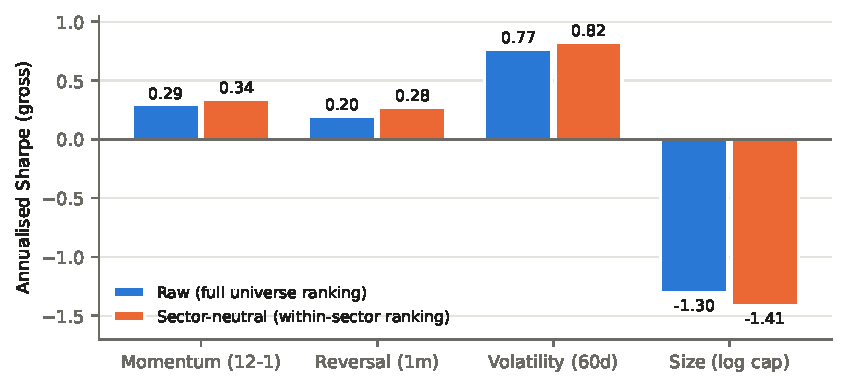
\includegraphics[width=\textwidth]{figures/sector_neutral_comparison.pdf}
\caption{Gross Sharpe ratio of raw and sector-neutral long-short portfolios.}
\label{fig:sector}
\end{figure}

\subsection{VIX regimes}

Table~\ref{tab:regimes} and Figure~\ref{fig:regimes} condition on the prior month's VIX. The directions are consistent with prior evidence: momentum's long-short return is negative after high-VIX months ($-0.45\%$ per month against $+0.55\%$ after low-VIX months), matching the rebound-crash mechanism, while high-volatility stocks and short-term reversal perform best after high-VIX months, when markets tend to rebound. However, none of the high-minus-low differences is statistically significant (Welch $p$-values between 0.06 and 0.78), which is unsurprising with about 58 months per tercile. These results are suggestive only.

\begin{table}[H]
\centering
\caption{Performance by tercile of the prior month-end VIX (cut-offs 14.8 and 18.2). Welch $t$-tests compare high- and low-VIX months.}
\label{tab:regimes}
\small
\tabfit{tables/regimes}
\end{table}

\begin{figure}[H]
\centering
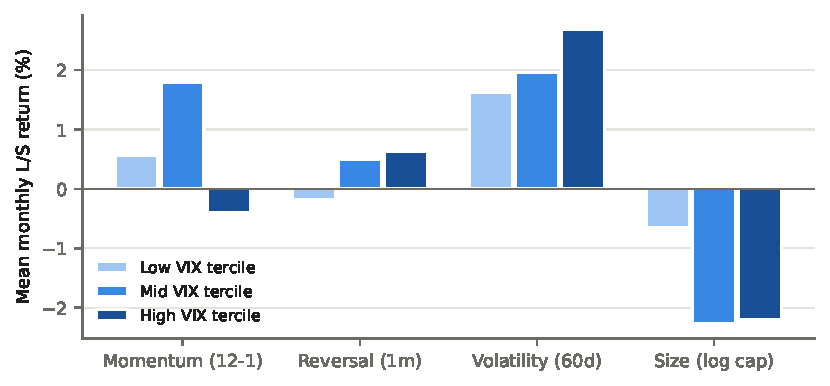
\includegraphics[width=\textwidth]{figures/vix_regimes.pdf}
\caption{Mean monthly long-short return by tercile of the prior month-end VIX.}
\label{fig:regimes}
\end{figure}

\section{Limitations}
\label{sec:limitations}

\textbf{Survivorship bias.} The universe consists of the 200 largest S\&P 500 members at the end of the sample. A company that was small in 2012 and is in this list in 2026 must have grown enormously, so the small-cap deciles are filled with ex post winners, and companies that shrank, were acquired or failed are absent entirely. This is the most likely explanation for the strongly negative size premium ($-21.26\%$ a year for the big-minus-small spread), which is the opposite of the conventional size effect and should not be read as evidence about size. The same bias inflates the average level of returns (the multivariate intercept implies roughly 1.7\% per month) and biases any factor correlated with the chance of ending the sample large: it favours high-variance stocks, which explains the positive residual volatility premium in Section~\ref{sec:risk}, and it is strongest near the selection date, which contributes to the concentration of raw premia in 2023 to 2026. Momentum may also be affected, since past winners that kept winning are more likely to be selected. A point-in-time constituent history (for example from CRSP) is required to remove the bias.

\textbf{Single-episode dependence and multiple testing.} The raw significance of momentum and volatility is concentrated in the 44 months from January 2023. Momentum's market-adjusted premium survives outside that period, but at $t = 2.49$ it falls short of the $t > 3$ hurdle that \citet{harvey2016} propose given the number of factors tested in the literature. The paper also reports several specifications per factor; conclusions are therefore drawn from agreement across specifications rather than from any single $t$-statistic.

\textbf{Risk model.} Risk adjustment uses a single factor (the market). Alphas against the Fama-French three- or five-factor models with momentum \citep{fama1993,carhart1997} would test whether the premia are explained by other known factors. Trailing betas are estimated with error from one year of daily data, which weakens beta as a control.

\textbf{Look-ahead in auxiliary data.} Market capitalisation uses the current share count for every month, and GICS sectors are current labels applied historically (for example, the 2018 reclassification that created Communication Services is not reflected). VIX tercile cut-offs use the full sample. None of these affects the return timing, but each uses information not available at the time.

\textbf{Sample size and power.} The study covers about 15 years of monthly data and 200 stocks, so roughly 20 stocks per decile. Decile portfolios are therefore noisy, the out-of-sample period has only 70 months, and the regime analysis only about 58 months per tercile.

\textbf{Transaction cost model.} Costs are a flat 10 basis points per unit of turnover. The model ignores market impact, bid-ask variation across stocks and over time, and the cost and availability of borrowing stocks for the short leg. It also ignores weight drift within each month, which understates true turnover.

\textbf{Portfolio construction.} Portfolios are equal-weighted and rebalanced monthly, which overweights the smaller names in the universe relative to a capacity-aware, value-weighted implementation. The long-short portfolios are not beta-neutral by construction; market exposure is removed only after the fact by regression, which a live strategy would have to achieve by hedging with estimated, and therefore imperfect, betas.

\textbf{Treatment of extremes.} Winsorising the factor characteristics compresses exactly the tail where, per \citet{daniel2016}, momentum's crash risk lives. The regression premia therefore describe a better-behaved factor than may exist. Rerunning the regressions on raw factors is a natural robustness extension.

\textbf{Scope.} The study omits established factors such as value, profitability and investment \citep{fama1993}, so the premia estimated here may partly proxy for these. Results for large U.S.\ stocks may not generalise to smaller stocks or other markets, particularly for short-term reversal, which is strongest among smaller, less liquid stocks.

\section{Conclusion}

Among the 200 largest current S\&P 500 constituents, 12-1 momentum and 60-day realised volatility both show positive and statistically significant raw Fama-MacBeth premia over 2012 to 2026 that are robust to sector neutralisation, and their break-even trading costs (56.0 and 193.0 basis points per unit turnover) are well above the assumed 10 basis points. Adjusting for market exposure separates them. The volatility premium is largely compensation for market beta in a strong bull market: the long-short portfolio has a beta of 1.17 and no alpha before 2023, and the regression premium disappears once the market is hedged. Momentum is close to market-neutral, and its market-adjusted premium of 3.7\% a year per standard deviation is significant over the full sample and before 2023, making it the most robust result in the study, in line with a large literature. Short-term reversal shows no reliable premium after costs. The strongly negative size premium, and a positive volatility premium in excess of beta that contradicts the literature, are attributed to survivorship bias in a universe selected at the end of the sample.

Important qualifications remain. Rank information coefficients are insignificant for both momentum and volatility, so their predictive content sits in the tails of the cross-section; momentum's decile alphas are only marginally significant; and no premium outside the 2023 to 2026 period clears the stricter $t > 3$ hurdle suggested for multiple testing.

The main value of the study lies in its process: a single, verified timing convention; three complementary evaluation lenses whose disagreements are explained rather than ignored; risk adjustment that distinguishes a factor premium from market exposure; and validation that identifies which results are artefacts of the sample. Natural extensions are a point-in-time, survivorship-free universe, a longer sample, alphas against multi-factor models, beta-neutral and value-weighted portfolios, value and profitability controls, and sub-industry neutralisation.

\section*{Reproducibility}

All code is in the project repository and runs in this order: \texttt{fetch\_universe.py}, \texttt{fetch\_market\_caps.py}, \texttt{fetch\_prices.py}, \texttt{fetch\_vix.py}, \texttt{fetch\_market.py}, \texttt{sanity\_check\_prices.py}, the five \texttt{compute\_*.py} factor and beta scripts, \texttt{check\_factor\_distributions.py}, \texttt{winsorize\_factors.py}, \texttt{decile\_backtest.py}, \texttt{fama\_macbeth.py}, \texttt{validation\_costs.py}, \texttt{extensions.py}, \texttt{risk\_adjustment.py}, \texttt{information\_coefficient.py}, \texttt{make\_figures.py} and \texttt{make\_tables.py}. Every table and figure in this paper is generated directly from the saved outputs, so no reported number is transcribed by hand.

\begin{thebibliography}{99}
\setlength{\itemsep}{2pt}
\small

\bibitem[Ang et~al.(2006)]{ang2006}
Ang, A., Hodrick, R.~J., Xing, Y., and Zhang, X. (2006). The cross-section of volatility and expected returns. \textit{Journal of Finance}, 61(1), 259--299.

\bibitem[Baker et~al.(2011)]{baker2011}
Baker, M., Bradley, B., and Wurgler, J. (2011). Benchmarks as limits to arbitrage: Understanding the low-volatility anomaly. \textit{Financial Analysts Journal}, 67(1), 40--54.

\bibitem[Banz(1981)]{banz1981}
Banz, R.~W. (1981). The relationship between return and market value of common stocks. \textit{Journal of Financial Economics}, 9(1), 3--18.

\bibitem[Carhart(1997)]{carhart1997}
Carhart, M.~M. (1997). On persistence in mutual fund performance. \textit{Journal of Finance}, 52(1), 57--82.

\bibitem[Daniel and Moskowitz(2016)]{daniel2016}
Daniel, K., and Moskowitz, T.~J. (2016). Momentum crashes. \textit{Journal of Financial Economics}, 122(2), 221--247.

\bibitem[Fama and French(1992)]{fama1992}
Fama, E.~F., and French, K.~R. (1992). The cross-section of expected stock returns. \textit{Journal of Finance}, 47(2), 427--465.

\bibitem[Fama and French(1993)]{fama1993}
Fama, E.~F., and French, K.~R. (1993). Common risk factors in the returns on stocks and bonds. \textit{Journal of Financial Economics}, 33(1), 3--56.

\bibitem[Fama and MacBeth(1973)]{fama1973}
Fama, E.~F., and MacBeth, J.~D. (1973). Risk, return, and equilibrium: Empirical tests. \textit{Journal of Political Economy}, 81(3), 607--636.

\bibitem[Frazzini and Pedersen(2014)]{frazzini2014}
Frazzini, A., and Pedersen, L.~H. (2014). Betting against beta. \textit{Journal of Financial Economics}, 111(1), 1--25.

\bibitem[Grinold and Kahn(2000)]{grinold2000}
Grinold, R.~C., and Kahn, R.~N. (2000). \textit{Active Portfolio Management} (2nd ed.). McGraw-Hill.

\bibitem[Harvey et~al.(2016)]{harvey2016}
Harvey, C.~R., Liu, Y., and Zhu, H. (2016). \ldots\ and the cross-section of expected returns. \textit{Review of Financial Studies}, 29(1), 5--68.

\bibitem[Jegadeesh(1990)]{jegadeesh1990}
Jegadeesh, N. (1990). Evidence of predictable behavior of security returns. \textit{Journal of Finance}, 45(3), 881--898.

\bibitem[Jegadeesh and Titman(1993)]{jegadeesh1993}
Jegadeesh, N., and Titman, S. (1993). Returns to buying winners and selling losers: Implications for stock market efficiency. \textit{Journal of Finance}, 48(1), 65--91.

\bibitem[Lehmann(1990)]{lehmann1990}
Lehmann, B.~N. (1990). Fads, martingales, and market efficiency. \textit{Quarterly Journal of Economics}, 105(1), 1--28.

\bibitem[McLean and Pontiff(2016)]{mclean2016}
McLean, R.~D., and Pontiff, J. (2016). Does academic research destroy stock return predictability? \textit{Journal of Finance}, 71(1), 5--32.

\bibitem[Newey and West(1987)]{newey1987}
Newey, W.~K., and West, K.~D. (1987). A simple, positive semi-definite, heteroskedasticity and autocorrelation consistent covariance matrix. \textit{Econometrica}, 55(3), 703--708.

\bibitem[Newey and West(1994)]{newey1994}
Newey, W.~K., and West, K.~D. (1994). Automatic lag selection in covariance matrix estimation. \textit{Review of Economic Studies}, 61(4), 631--653.

\bibitem[Novy-Marx and Velikov(2016)]{novymarx2016}
Novy-Marx, R., and Velikov, M. (2016). A taxonomy of anomalies and their trading costs. \textit{Review of Financial Studies}, 29(1), 104--147.

\bibitem[Sharpe(1964)]{sharpe1964}
Sharpe, W.~F. (1964). Capital asset prices: A theory of market equilibrium under conditions of risk. \textit{Journal of Finance}, 19(3), 425--442.

\end{thebibliography}

\end{document}
